\documentclass[border=10pt]{standalone}
\usepackage{tikz}
\usetikzlibrary{shapes.geometric, arrows.meta, positioning, calc, shadows}
\usepackage{xcolor}

% Color palette
\definecolor{primaryblue}{HTML}{0056B3}
\definecolor{secondarygrey}{HTML}{F8F9FA}
\definecolor{bordergrey}{HTML}{DDDDDD}
\definecolor{textdark}{HTML}{333333}
\definecolor{texthighlight}{HTML}{FFFFFF}
\definecolor{datagreen}{HTML}{28A745}

\begin{document}

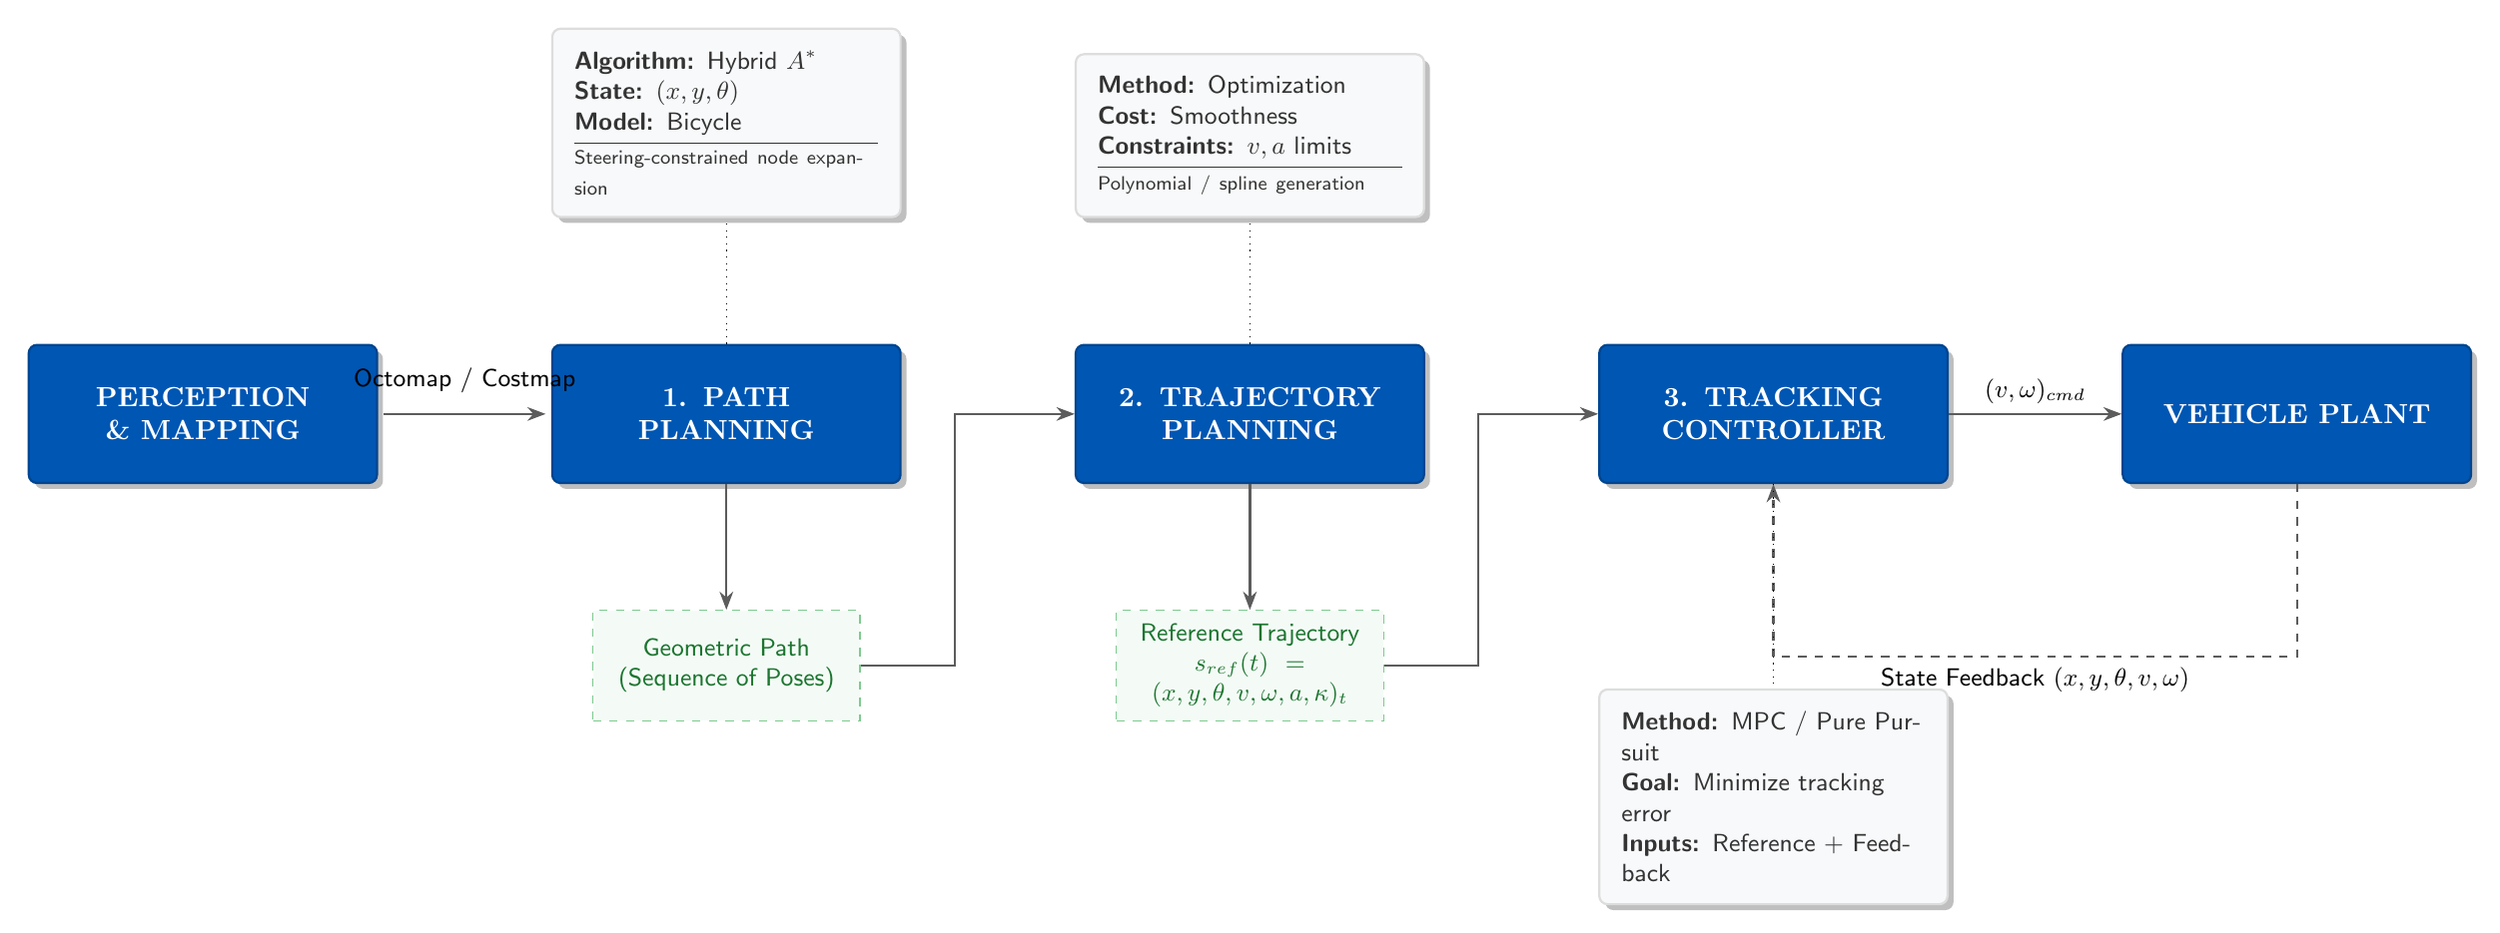
\begin{tikzpicture}[
    font=\sffamily\small,
    node distance=2.8cm and 2.2cm,
    block/.style={
        rectangle, draw=bordergrey, thick,
        fill=secondarygrey,
        text width=11em,
        minimum height=5em,
        rounded corners=3pt,
        align=left,
        text=textdark,
        inner sep=8pt,
        drop shadow
    },
    major/.style={
        block,
        fill=primaryblue,
        draw=primaryblue!80!black,
        text=white,
        font=\bfseries,
        align=center
    },
    data/.style={
        rectangle,
        draw=datagreen!60,
        dashed,
        fill=datagreen!5,
        text width=9em,
        minimum height=4em,
        align=center,
        text=datagreen!70!black
    },
    arr/.style={
        -{Stealth},
        thick,
        draw=textdark!80
    }
]

% ==========================================
% CORE PIPELINE
% ==========================================

\node[major] (start) {PERCEPTION \& MAPPING};
\node[major, right=of start] (path) {1. PATH PLANNING};
\node[major, right=of path] (traj) {2. TRAJECTORY\\ PLANNING};
\node[major, right=of traj] (ctrl) {3. TRACKING\\ CONTROLLER};
\node[major, right=of ctrl] (plant) {VEHICLE PLANT};

% ==========================================
% DATA LAYER
% ==========================================

\node[data, below=1.6cm of path] (geopath)
{Geometric Path\\(Sequence of Poses)};

\node[data, below=1.6cm of traj] (reftraj)
{Reference Trajectory\\
$s_{ref}(t) = (x,y,\theta,v,\omega,a, \kappa)_t$};

% ==========================================
% MAIN CONNECTIONS
% ==========================================

% Clean label placement (no overlap)
\draw[arr, shorten >=2pt, shorten <=2pt]
(start) -- node[above=4pt] {Octomap / Costmap} (path);

\draw[arr] (path) -- (geopath);

% Routed Geopath → Trajectory (no crossing)
\coordinate (mid1) at ($(geopath.east)+(1.2,0)$);
\draw[arr] (geopath.east) -- (mid1) |- (traj.west);

\draw[arr] (traj) -- (reftraj);

% Routed Ref → Controller (no crossing)
\coordinate (mid2) at ($(reftraj.east)+(1.2,0)$);
\draw[arr] (reftraj.east) -- (mid2) |- (ctrl.west);

\draw[arr] (ctrl) -- node[above] {$(v, \omega)_{cmd}$} (plant);

% ==========================================
% FEEDBACK LOOP
% ==========================================

\coordinate (fb1) at ($(plant.south)+(0,-2.2)$);

\draw[arr, dashed]
(plant.south) -- (fb1)
-| node[pos=0.25, below]
{State Feedback $(x,y,\theta,v, \omega)$}
(ctrl.south);

% ==========================================
% ANNOTATION LAYER (TOP)
% ==========================================

\node[block, above=1.6cm of path] (path_det) {
\textbf{Algorithm:} Hybrid $A^*$\\
\textbf{State:} $(x,y,\theta)$\\
\textbf{Model:} Bicycle\\
\vspace{0.3em}\hrule\vspace{0.3em}
\scriptsize Steering-constrained node expansion
};

\draw[dotted] (path.north) -- (path_det.south);

\node[block, above=1.6cm of traj] (traj_det) {
\textbf{Method:} Optimization\\
\textbf{Cost:} Smoothness\\
\textbf{Constraints:} $v,a$ limits\\
\vspace{0.3em}\hrule\vspace{0.3em}
\scriptsize Polynomial / spline generation
};

\draw[dotted] (traj.north) -- (traj_det.south);

% ==========================================
% CONTROLLER DETAILS (LOWERED)
% ==========================================

\node[block, below=2.6cm of ctrl] (ctrl_det) {
\textbf{Method:} MPC / Pure Pursuit\\
\textbf{Goal:} Minimize tracking error\\
\textbf{Inputs:} Reference + Feedback
};

\draw[dotted] (ctrl.south) -- (ctrl_det.north);

\end{tikzpicture}

\end{document}